\documentclass[10pt,twocolumn,letterpaper]{article}

\usepackage{cvpr}
\usepackage{times}
\usepackage{epsfig}
\usepackage{graphicx}
\usepackage{amsmath}
\usepackage{amssymb}

\usepackage{media9}
\usepackage{filecontents}
%\usepackage{geometry}
\usepackage{caption}
\usepackage{subcaption}

% Include other packages here, before hyperref.

% If you comment hyperref and then uncomment it, you should delete
% egpaper.aux before re-running latex.  (Or just hit 'q' on the first latex
% run, let it finish, and you should be clear).
\usepackage[breaklinks=true,bookmarks=false]{hyperref}

\cvprfinalcopy % *** Uncomment this line for the final submission
\def\httilde{\mbox{\tt\raisebox{-.5ex}{\symbol{126}}}}

% Pages are numbered in submission mode, and unnumbered in camera-ready
%\ifcvprfinal\pagestyle{empty}\fi
\setcounter{page}{1}
\begin{document}

%%%%%%%%% TITLE
\title{Volumetric Capture}

\author{Marcel Bruckner\\
{\tt\small marcel.bruckner@tum.de}
\and
Kevin Bein\\
{\tt\small kevin.bein@tum.de}\\[0.5em]
Technical University of Munich
\and
Moiz Sajid\\
{\tt\small moiz.sajid@tum.de}
}

\maketitle
%\thispagestyle{empty}

%%%%%%%%% ABSTRACT
\begin{abstract}
   Our goal in this project is to get a realtime mesh reconstruction of dynamic scenes using a multi view camera capture setup. We use three Intel RealSense D415 depth cameras for RGB-D data capturing which are calibrated using known correspondences from markers. The data is fused into a voxelgrid representing the implicit surface and following a marching cubes algorithm is performed for the final surface extraction. Both qualitative and quantitative results are presented in this report.   
\end{abstract}


\begin{figure}[t]
	\begin{center}
		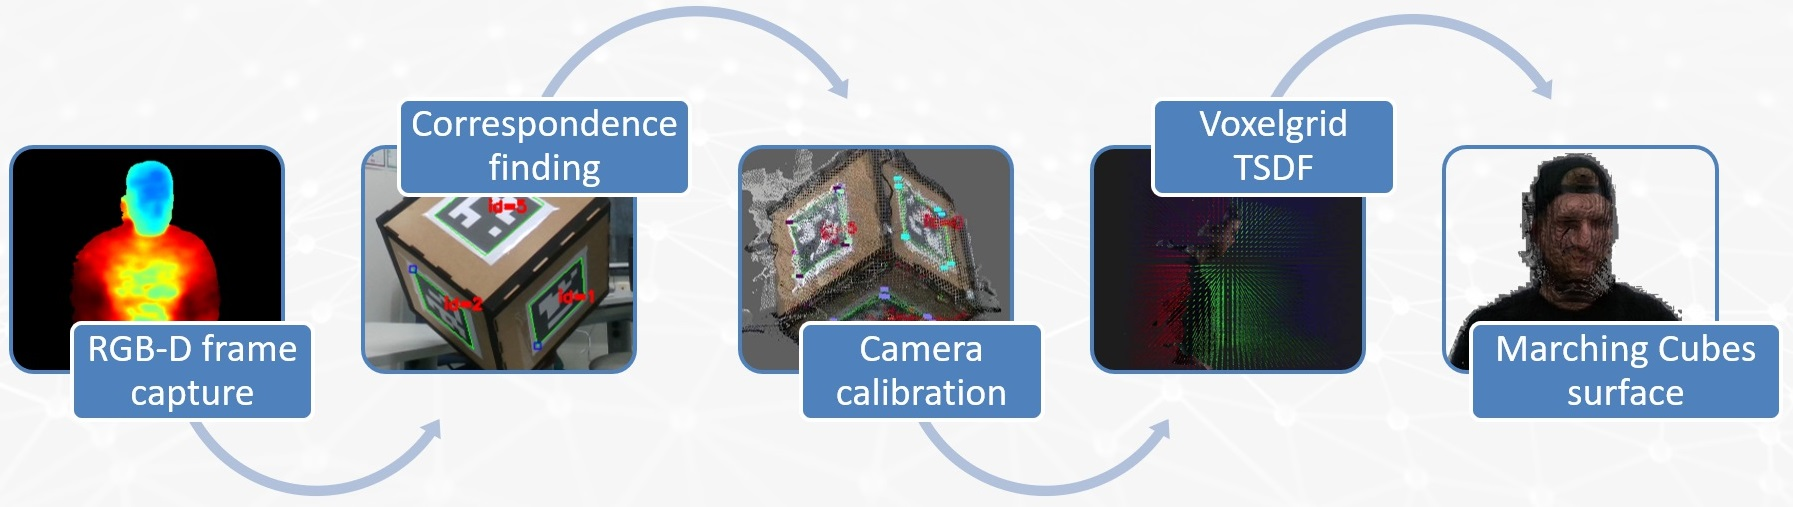
\includegraphics[width=1.0\linewidth]{imgs/pipeline}
	\end{center}
	\caption{Reconstruction pipeline used in this project: RGB-D Frame Capture, Correspondence Finding, Camera Calibration, Voxelgrid TSDF, Marching Cubes}
	\label{fig:long}
	\label{fig:onecol}
\end{figure}

%%%%%%%%% BODY TEXT
\section{Introduction}

Volumetric Capture is an extensively researched topic where the ultimate goal is to get an accurate 3D reconstruction in realtime. The first work in the area was done Cureless and Levoy~\cite{Authors4} in which they integrated data from one range image into cumulative weighted signed distance function. KinectFusion~\cite{Authors5} was another milestone in this area which proposed a realtime mapping system of indoor scenes using a single depth camera. DynamicFusion~\cite{Authors6} handles non-rigid scenes but our work mostly focussed on handling rigid scenes. 

One of application areas of our project is Holoportation~\cite{Authors7} where 3D recontructed models were used for interactions between two persons using Microsoft HoloLens.

%------------------------------------------------------------------------
\section{Reconstruction Pipeline}


%-------------------------------------------------------------------------
\subsection{RGB-D Frame Capture}
We used three D415 Intel RealSense cameras for our capture setup. One of the benefits of using Intel RealSense cameras is that it provides good support and updates for its API. The Intel RealSense cameras work on the concept of Active Stereo in which a texture in projected for better better details. The RGB-D frames from the three cameras were time synchronized which not only helped us to get better results for the cameras calibration but also for the final mesh reconstruction. For depth image preprocessing, we used Threshold Filtering in which the depth of the objects that are a certain distance away from the camera get discarded.

\begin{figure}
  \centering
  \begin{subfigure}[t]{.315\linewidth}
    \centering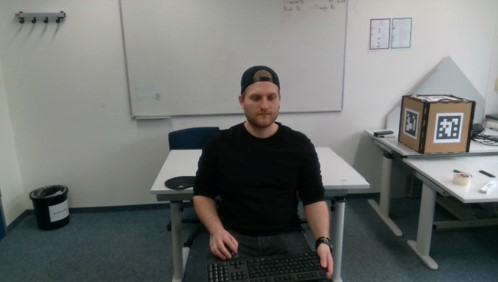
\includegraphics[width=0.9\linewidth]{imgs/rgb}
    \caption{RGB Image}
    \label{fig:rgb}
  \end{subfigure}
  \begin{subfigure}[t]{.315\linewidth}
    \centering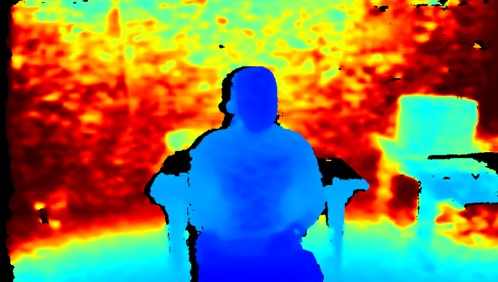
\includegraphics[width=0.9\linewidth]{imgs/depth}
    \caption{Depth Image}
    \label{fig:depth}
  \end{subfigure}
  \begin{subfigure}[t]{.315\linewidth}
    \centering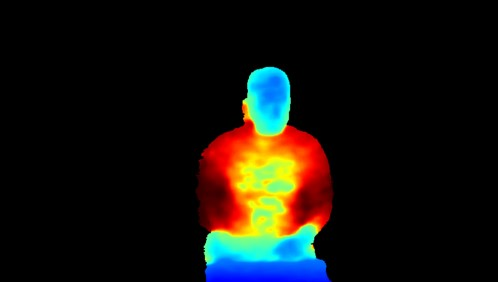
\includegraphics[width=0.9\linewidth]{imgs/threshold}
    \caption{Threshold Filtered Image}
    \label{fig:threshold}
  \end{subfigure}  
  \caption{ }
\end{figure}

For further filtering, we also tried using Hole Filing for ending gaps in the depth images, Spatial Filtering for smoothing the edges and Edge Enhancement Filter. All of these filters did not led to any significant improvements hence they were not used in the final mesh reconstruction. For captur setup, we initally wanted to use four camera but due to bandwidth limitations we were not able to use color and the depth streams from all four cameras at the same time instance. We also had to limit the color and depth frame resolution for faster processing. The resolution which we used for the color stream is 848 by 480 pixels and for the depth stream is 848 by 480 pixels.

\begin{figure}[t]
\begin{center}
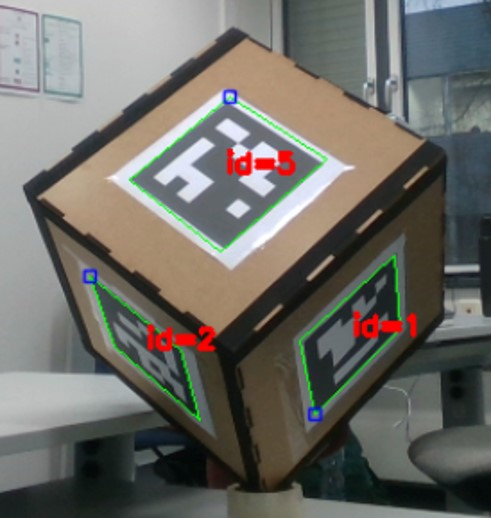
\includegraphics[width=0.6\linewidth]{imgs/cube}
\end{center}
 \caption{ArUco box cube with the detected marker identifiers. The markers were used for camera calibration}
 \label{fig:cube}
\end{figure}
  
%-------------------------------------------------------------------------
\subsection{Correspondence Finding}
For correspondences, we used ArUco markers with each marker having a unique identifier. The markers were mounted on a cube box as shown in Figure \ref{fig:cube}. The markers were placed in such a way such that any one particular camera can easily detect two out of three markers. The cameras placed with significant view overlap. In the end, we just opted for one marker per side. It is also important to mention here that we also tried the ChArUco markers which is basically a chessboard with the ArUco markers. However, the ChArUco markers did not gave us good results. 

%-------------------------------------------------------------------------
\subsection{Camera Calibration}
After getting the marker locations, we backprojected these correspondences into the 3D pointcloud using the depth information. The camera poses of the cameras were then estimated using OpenCV. Using these camera poses, we calculated relative transformatons between the cameras. Out of three camera, we selected the first camera's coordinate frame as the world coordinate frame and hence the poses from the other two cameras were aligned with respect to the first camera. The alignment we got from the camera calibration was not good which meant that it can be improved further.

%-------------------------------------------------------------------------
\subsection{Optimization}
As the pose parameters that we got from the camera calibration were not good enough, we used two different optimizations approaches namely Procrutes and Point-to-Point correspondence error for optimizing the 3D pose parameters of the cameras even further.
 
In the Procrustes algorithm, we compute the vector between the center of gravity for getting the translation components and the Singular Value Decomposition of the known correspondences for getting the rotation components as shown in Equation (\ref{eq3}) and (\ref{eq4}). The alignment that we get from Procrustes is not robust enough and hence has a high Mean Squared Error (MSE).\\

\begin{equation}\label{eq3}
USV^T=SVD(X^TX)
\end{equation}

\begin{equation}\label{eq4}
R=UV^T
\end{equation}

In order to further improve the results that we get from Procrustes, we used the Point-to-Point correspondence error. For the Point-to-Point correspondence error, we optimize for the following energy term:

\begin{equation}\label{eq5}
\sum_{i}\sum_{j}\sum_{k} \left\Vert\left(X_{ik} - T_jR_j*X_{jk}\right)\right\Vert_2^2
\end{equation}

Further results have been sumarzied in Table~\ref{tab:table1}. One of the difficulties that we faced in camera calibration was visualizing the aligned points for which we had to write our own rendering pipeline in OpenGL~\cite{Authors3}. Another difficulty that we faced was with Ceres because we had to get ourselves acquainted with general working of the non-linear optimization framework. 
%-------------------------------------------------------------------------
\subsection{Voxelgrid TSDF}
Once we have these aligned pointclouds, we fuse them into the voxelgrid. We project the voxelgrid into the depth frame of the camera and we calculate the difference by subtracting the voxel depth from the actual depth value using Equation (\ref{eq1}). For the truncated signed-distance function (tsdf) values we did the weighted averaging using the Equation (\ref{eq2}). The tsdf values were truncated between -1 and 1 with points having a negative value inside the surface and positive value outside the surface.

\begin{equation}\label{eq1}
tsdf=z_{voxel} - z_{depth}
\end{equation}

\begin{equation}\label{eq2}
tsdf_{i+1}=\frac{tsdf_{i} * weight}{weight+1}
\end{equation}

Given that we were using a large number of gridpoints, computing tsdf values on the CPU was not feasible. So we had to move our tsdf voxelgrid implementation onto the GPU inorder to achieve realtime results. Since we were already using OpenGL for the rendering pipeline, we decided to use OpenGL Compute Shaders~\cite{Authors1} for parallelizing the tsdf voxelgrid implementation. We also had to find a tradeoff between voxel resolution and frame rate. With a lower voxel resolution, the frame rate dropped because more calculations had to be done. Furthermore, finding a good truncation distance was also very crucial for lowering the artefacts. The Table~\ref{tab:table2} summarizes the time comparisons between different voxel resolutions.

\begin{figure}[t]
\begin{center}
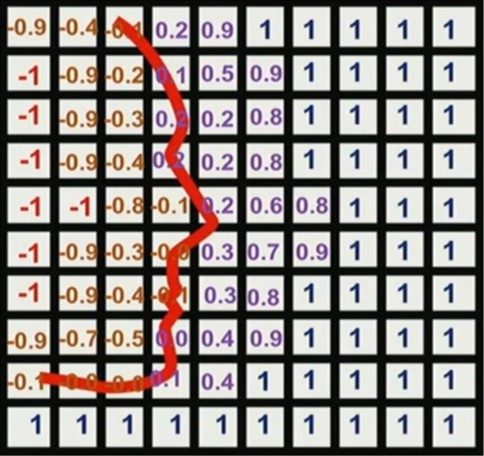
\includegraphics[width=0.6\linewidth]{imgs/tsdf}
\end{center}
 \caption{TSDF Represenation}
\end{figure}

%-------------------------------------------------------------------------
\subsection{Surface Extraction}
For the iso-surface extraction, we used the Marching Cubes algorithm which converts the implicit surface representation to a polygonal mesh. We then iterated over the voxelgrid cells to determine the zero crossings and looked up the triangulation in the Marching Cubes table. This gives us the trianguled mesh as an final output. With a lower voxel resolution and more grid points, we were able to get more finer reconsturction. Again we had to utilize the OpenGL Compute Shader in order to achieve realtime results because the computations on the CPU were really slow.

Intially, we had voxelgrid points that were not initialized because they were outside the camera view. As a result, we had a huge number of artefacts in the final mesh reconstruction which took a lot of time to figure out. We implemented a two pass OpenGL Compute Shader. In the first pass, we counted the number of triangles that will generated and only allocated space for them. In the second pass, we generate the triangles. We do this because the upper bound for the number of generated triangle is five times the number of voxelgrid points. For example if we have 200x200x200 grid points with a 5 millimeter voxel resolution, we roughly had 40 million number of possible triangles. We only generated a fraction of these triangles after the the triangle counting OpenGL Compute Shader pass. For a voxel resolution of 5mm resolution, the Marching Cubes algorithm took 15 milliseconds which was realtime capable. For 3 millimeter resolution, the results were not realtime capable however, we were to get fine mesh reconstructions.  The Table~\ref{tab:table2} summarizes the time comparisons between different voxel resolution. The Table~\ref{tab:table3} summarizes the time comparisons for running Marching Cubes between different voxel resolutions. 

%------------------------------------------------------------------------
\section{Results}
The results that we get using one camea are really good as can be seen in Figure \ref{fig:res1}. Figure \ref{fig:res2} displays the triangulation results using one camera. However, we get artefacts when we use all three camera streams. The which artefacts which are mostly visible around the edges can be seen in Figure \ref{fig:res3}. This suggests that the camera pose parameters can be improved further.

\begin{figure}[t]
\begin{center}
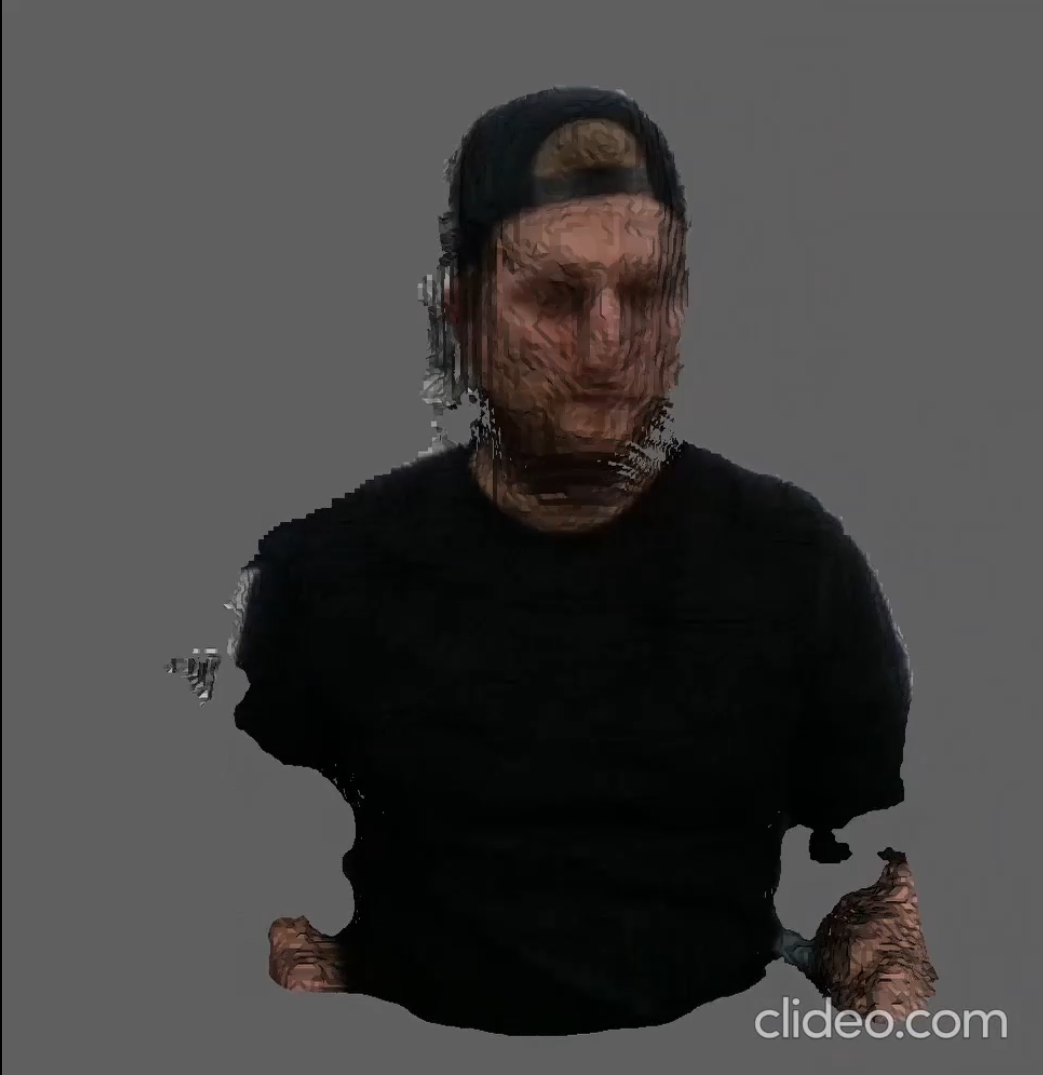
\includegraphics[width=0.65\linewidth]{imgs/res1}
\end{center}
 \caption{Result with using only one camera}
 \label{fig:res1}
\end{figure}

\begin{figure}[t]
\begin{center}
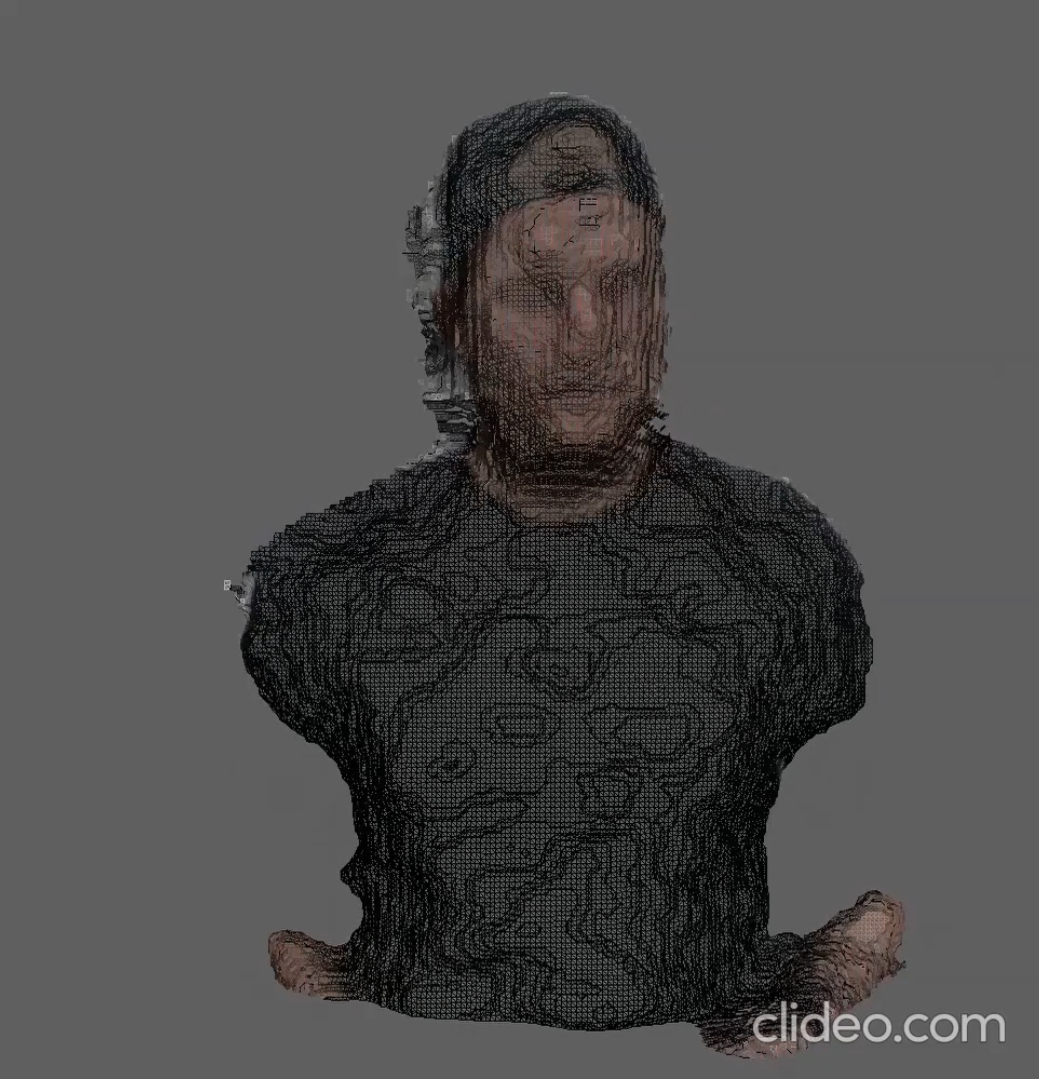
\includegraphics[width=0.65\linewidth]{imgs/res2}
\end{center}
 \caption{Triangulation result with using only one camera}
 \label{fig:res2}
\end{figure}

\begin{figure}[t]
\begin{center}
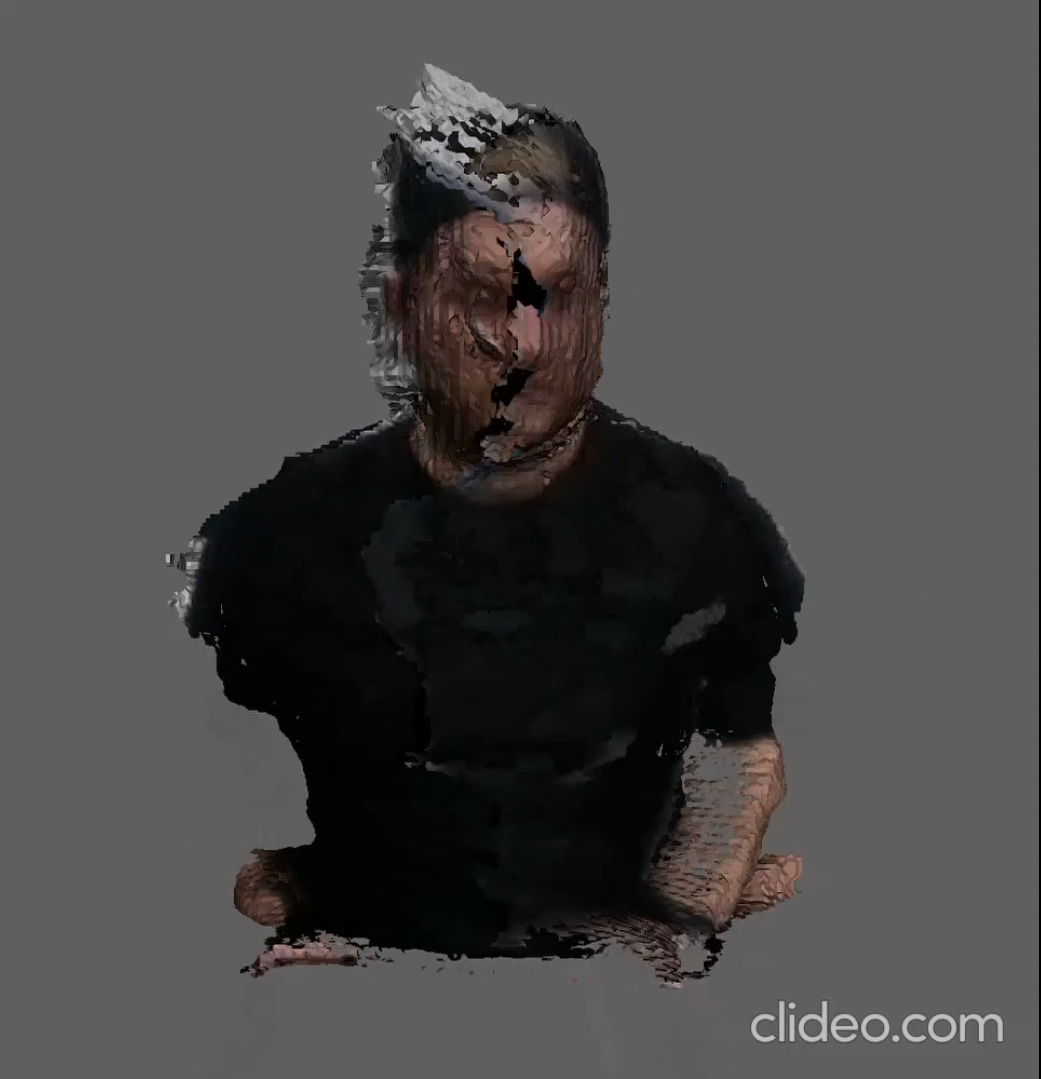
\includegraphics[width=0.65\linewidth]{imgs/res3}
\end{center}
 \caption{Result with using three cameras}
 \label{fig:res3}
\end{figure}

\begin{table}[h!]
  \begin{center}
    \begin{tabular}{c|c|c|c p{4cm}}
      \textbf{Algorithm} & \textbf{Iterations} & \textbf{Duration [ms]} & \textbf{MSE}\\
      \hline
      Procrustes (A)  & 1 & 8 - 20 & \textless 0.7 - 1.73\\
      Point-to-Point (A) & 1 - 20 & 900 - 1000 & \textless 0.1\\
      Procrustes (C) & 1 & 20 - 40 & 0.25 - 1.29\\
      Point-to-Point (C) & 1 - 20 & 18000 - 22000 & \textless 0.1\\
    \end{tabular}
     \caption{Comparisons between different optimization algorithms in terms of iterations, duration and MSE (Mean Squared Error). A=ArUco and C=ChArUco}
     \label{tab:table1}
  \end{center}
\end{table}

\begin{table}[h!]
  \begin{center}
    \begin{tabular}{c|c|c|c p{4cm}}
      \textbf{Algorithm} & \textbf{Resolution [mm]} & \textbf{Gridpoints} & \textbf{Duration [ms]}\\
      \hline
      All frames & 20 & 125,000 & \textless 1\\
      All frames & 10 & 1,000,000 & \textless 1\\
      All frames & 5 & 8,000,000 & 5\\
      All frames & 4 & 15,625,000 & 20\\
      All frames & 3 & 37,000,000 & 50\\
    \end{tabular}
     \caption{Time comparisons for calculating voxelgrid of different voxel resolutions as well as the number of gridpoints used. The voxelgrid measured 1 meter x 1 meter x 1 meter.}
     \label{tab:table2}
  \end{center}
\end{table}

\begin{table}[h!]
  \begin{center}
    \begin{tabular}{c|c|c p{4cm}}
      \textbf{Resolution [mm]} & \textbf{Duration [ms]} & \textbf{Gridpoints}\\
      \hline
      20 & \textless 1 & 7,000 - 10,000\\
      10 & \textless 1 & 40,000 - 45,000\\
      5 & 15 & 200,000 - 250,000\\
      4 & 35 & 380,000 - 420,000\\
      3 & 80 & 600,000 - 800,000\\
    \end{tabular}
     \caption{Time comparisons for running the Marching Cubes on different voxel resolutions. The number of triangles generated are also displayed.}
     \label{tab:table3}
  \end{center}
\end{table}

%------------------------------------------------------------------------
\section{Future Work and Conclusion}
Since we optimized for pose parameters for a limited number of markers, one of the further improvements that we can do in camera calibration is to use more correspondences which can found for example by using Nearest Neighbor Search and then use the Global Alignment techniques like Iterative Closest Points (ICP).

%------------------------------------------------------------------------
\section{Group Member Contributions}

{\small
\bibliographystyle{ieee_fullname}
\bibliography{egbib}
}

\end{document}
